\documentclass{article}

\usepackage[left=2cm,right=2cm,top=2cm,bottom=2cm]{geometry} 

\usepackage[utf8]{inputenc}   % otra alternativa para los caracteres acentuados y la "ñ"
\usepackage[           spanish % para poder usar el español
                      ,es-tabla % para los captions de las tablas
                       ]{babel}   
\decimalpoint %para usar el punto decimal en vez de coma para los números con decimales

%\usepackage{beton}
%\usepackage[T1]{fontenc}

\usepackage{parskip}
\usepackage{xcolor}

\usepackage{caption}

\usepackage{enumerate} % paquete para poder personalizar fácilmente la apariencia de las listas enumerativas

\usepackage{graphicx} % figuras
\usepackage{subfigure} % subfiguras

\usepackage{amsfonts}
\usepackage{amsmath}

\usepackage{listings}
\lstset
{ %Formatting for code in appendix
    language=python,
    basicstyle=\footnotesize,
    stepnumber=1,
    showstringspaces=false,
    tabsize=1,
    breaklines=true,
    breakatwhitespace=false,
}

\definecolor{gris}{RGB}{220,220,220}
	
\usepackage{float} % para controlar la situación de los entornos flotantes

\restylefloat{figure}
\restylefloat{table} 
\setlength{\parindent}{0mm}


\usepackage[bookmarks=true,
            bookmarksnumbered=false, % true means bookmarks in 
                                     % left window are numbered
            bookmarksopen=false,     % true means only level 1
                                     % are displayed.
            colorlinks=true,
            allcolors=blue,
            urlcolor=blue]{hyperref}
\definecolor{webblue}{rgb}{0, 0, 0.5}  % less intense blue

\usepackage[ruled,vlined]{algorithm2e}
\SetKwInOut{Parameter}{parameter}
\newcommand{\Or}{\textbf{ or }}
\renewcommand{\And}{\textbf{ and }}


\title{\Huge Metaheurística: Práctica Alternativa al Examen \\ Búsqueda Ramificada con Momentos \vspace{10mm}}

\author{\huge David Cabezas Berrido \vspace{10mm} \\
	\huge 20079906D \vspace{10mm} \\  
  \huge Grupo 2: Viernes \vspace{10mm} \\ 
  \huge dxabezas@correo.ugr.es \vspace{10mm}}

\begin{document}
\maketitle
\newpage
\tableofcontents
\newpage

\section{Descripción de la Metaheurística}

Nuestro problema es la optimización continua de una serie de funciones. Estamos limitados por el número de evaluaciones, que en nuestro
caso será 10000 multiplicado por la dimensión del espacio de soluciones.

Diseñaremos nuestra propia metaheurística y la pondremos a prueba con el benchmark CEC'2017. Por tanto, nuestro objetivo es la optimización de parámetros
reales. Con nuestra propuesta esperamos alcanzar un buen compromiso entre exploración y explotación aprovechando la naturaleza continua del espacio
de soluciones.

\subsection{Idea general}
Nuestra metaheurística, \textbf{Búsqueda Ramificada con Momentos}, pretende ``lanzar'' soluciones que se muevan por el espacio como lo harían bombas
lanzadas desde un avión bombardeos, fragmentos que se desprenden de un cuerpo celeste o el despliegue de una sonda de una nave espacial.
Es decir, se explora el espacio ramificando o dividiendo las soluciones en otras, de
forma que las soluciones resultantes conserven la inercia de la solución de la que partieron.

\begin{figure}[H]
	\centering
	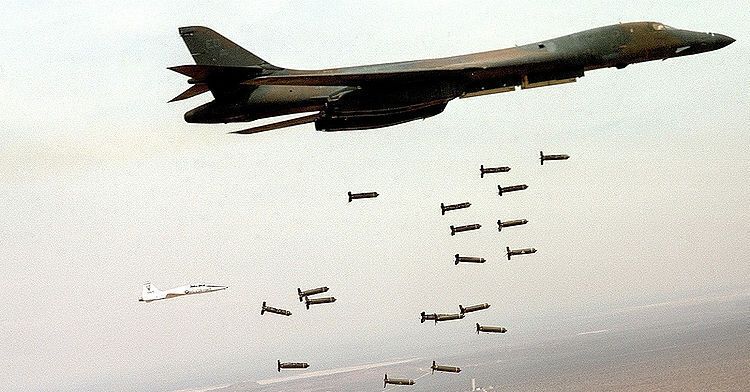
\includegraphics[width=140mm]{imgs/bombs}
	\caption{Cuando se despliegan bombas desde un avión, las bombas mantienen la inercia del movimiento del avión.}
\end{figure}

Para dar sentido a este fenómeno físico que es la conservación de la inercia ideamos una estrategia de explotación basada en momentos, similar
a la Búsqueda Local salvo que se pondera el momento de la solución con la dirección de un vecino mejor.

Las soluciones pueden ser truncadas bajo ciertas
condiciones, así que se van lanzando nuevas soluciones desde puntos aleatorios hasta agotar el número máximo de evaluaciones.

\subsection{Explicación del algoritmo}

El algoritmo comienza con una solución aleatoria, un vector aleatorio de flotantes, $S$. Cada solución tiene asociado otro vector aleatorio que es
su momento, $\nu$, que intuitivamente se puede interpretar como la dirección en la que se está moviendo la solución actualmente; también tiene un
valor escalar positivo, $\lambda$ que podría interpretarse como un impulso, la solución se desplaza usando su momento y su impulso:
$S\gets S+\lambda\nu$.

Cada solución tiene un número determinado de evaluaciones. En cada iteración, una solución puede hacer una de las siguientes acciones:
\begin{itemize}
	\item La solución desaparece, es truncada.
	\item La solución se divide en dos, que ``saldrán disparadas'' en direcciones opuestas.
	\item La solución desvía su dirección hacia un vecino del entorno con mejor fitness y luego se actualiza usando su impulso y su momento: $S\gets S+\lambda\nu$. La solución pierde una cantidad de impulso determinada por el éxito de la búsqueda de un vecino mejor en el entorno.
\end{itemize}
La acción a realizar en cada momento depende de la fitness de la solución respecto a la mejor fitness encontrada hasta el momento, del número de evaluaciones restantes y del impulso que le quede a la solución. Queremos truncar soluciones que no tengan muchas posibilidades de mejorar, ya sea porque
estén muy lejos de la mejor hasta el momento y les queden pocas iteraciones o porque su impulso sea prácticamente nulo. Queremos dividir soluciones
que sean de las mejores, tengan bastantes evaluaciones por delante y no acaben de ser lanzadas desde otras, para evitar que haya soluciones muy
cercanas entre sí.

Estos objetivos pueden ser muy difíciles de lograr debido al número de factores a tener en cuenta, a continuación presentamos nuestro intento de
lograr un equilibrio.

\subsubsection*{Decisión de la acción}

En nuestro caso, primero tomaremos la diferencia entre la fitness de la solución y la mejor fitness encontrada hasta el momento: $D\gets fitness-best$.
Como estamos minimizando, será una cantidad no negativa. En principio tenemos $D\in[0,+\infty[$, para normalizar la escala utilizamos una función
creciente que identifique este intervalo con el $[0,1[$, $\hat{D}\gets \dfrac{D}{1+D}$.

Decidimos truncar la solución cuando esta diferencia sea alta y
las posibilidades de mejorarla sean escasas, ya sea por que la solución tenga pocas evaluaciones restantes o porque su impulso sea bajo.

Decidimos ramificar la solución en dos cuando esta diferencia sea baja, el impulso esté en un rango determinado (no queremos dividir ni muy pronto ni
muy tarde) y el número de evaluaciones restantes sea suficiente para que las soluciones resultantes puedan mejorar.

En el resto de casos, la solución se limita a avanzar.

En nuestra implementación, hemos decidido dar esta estructura al bucle principal, que combina las ideas anteriores con una componente aleatoria.

 \begin{algorithm}[H]
	\DontPrintSemicolon % Some LaTeX compilers require you to use \dontprintsemicolon instead
	\KwIn{Una solución: vector de flotantes $S$}
	\KwIn{Su momento: vector de flotantes $\mu$}
	\KwIn{Su impulso: escalar positivo $\lambda$}
	\KwIn{Evaluaciones a realizar: entero positivo $evals$}
	$fitness\gets \operatorname{eval}(S)$ \tcp*{Supondremos la función de evaluación siempre disponible}
	$evals\gets evals-1$\;
	$best\gets\operatorname{min}(best, fitness)$\;
	\While{$evals>0$}{
		$D\gets fitness-best$ \tcp*{Suponemos accesible la mejor fitness obtenida hasta el momento}
		$\hat{D}\gets \frac{D}{1+D}$ \tcp*{Diferencia normalizada en $[0,1[$}
		$p\gets U[0,1]$ \tcp*{Flotante aleatorio en $[0,1]$, elegido según la distribución uniforme}
		\If{$(p<P_{vanish}\frac{\hat{D}}{\lambda} \And evals\leq MaxEvalsTruncate) \Or \lambda < MinImpulse$}{
			\text{La solución es truncada.}
		}
		\ElseIf{$p>P_{split}\frac{\hat{D}}{\lambda} \And MinImpulseSplit\leq\lambda\leq MaxImpulseSplit \And evals\geq MinEvalsSplit$}{
			\text{La solución se divide en dos.}
		}
		\Else{La solución avanza.}
	}
	\caption{{\sc Branch:} Búsqueda Ramificada: Bucle Principal.}
	\label{alg:branch}
\end{algorithm}

Más adelante discutiremos los parámetros que han aparecido a lo largo del algoritmo. De momento nos centraremos en detallar cada una de las
acciones que aparecen en el bucle.

\subsubsection*{Truncamiento de la solución}
Cuando una solución es truncada, simplemente se corta el bucle con la orden \textbf{break}. Antes, hay que acumular las evaluaciones a
realizar para que no se desperdicien, las llamadas restantes se acumulan para mejorar futuras soluciones: $spareEvals\gets spareEvals+evals$.

\subsubsection*{Ramificación de la solución}

Cuando una solución se ramifica, se generan dos soluciones con empujes opuestos desde ella y se acumulan los momentos. Además, se
recargan en cierta proporción del impulso perdido desde el inicial, $\lambda_0$. Las evaluaciones pendientes se reparten equitativamente
entre las dos soluciones generadas, como la división es entera, se rescata la evaluación sobrante en caso de que el número de evaluaciones
sea impar. La solución es destruida, ya que se queda sin evaluaciones.

 \begin{algorithm}[H]
	\DontPrintSemicolon % Some LaTeX compilers require you to use \dontprintsemicolon instead
	$modification\gets\text{vector aleatorio, las componentes se generan con una $U[0,1]$}$\;
	$\mu_1\gets \mu + modification$ \tcp*{Las soluciones salen en direcciones opuestas}
	$\mu_2\gets \mu - modification$\;
	$\lambda_1\gets \lambda+SplitImpulse\cdot(\lambda_0-\lambda)$ \tcp*{Se recarga parcialmente el impulso}
	$\lambda_2\gets \lambda+SplitImpulse\cdot(\lambda_0-\lambda)$\;
	$S_1 \gets S+\lambda_1 \mu_1$\;
	$S_2 \gets S+\lambda_2 \mu_2$\;
	$\operatorname{clip}(S_1)$ \tcp*{Si alguna componente se sale del rango, se fija en el borde}
	$\operatorname{clip}(S_2)$\;
	\If{$evals \% 2 = 1$}{
		$spareEvals\gets spareEvals+1$ \tcp*{Para evitar perder evaluaciones}
	}
	$\operatorname{branch}(S_1, \mu_1, \lambda_1, evals/2)$\;
	$\operatorname{branch}(S_2, \mu_2, \lambda_2, evals/2)$\;
	\textbf{break} \tcp*{Esta solución desaparece}
	\caption{{\sc Split:} Ramificación de una solución $S$ como la de entrada del Algoritmo \ref{alg:branch}.}
	\label{alg:split}
\end{algorithm}

\subsubsection*{Avance de la solución}
Para el avance de la solución se buscan vecinos aleatorios en un entorno de la solución, para mí siempre se tiene $\lambda\in]0,1]$ y he escogido radio $\sqrt{\lambda}$. Si se encuentra un vecino mejor en un determinado número de intentos, se considera un éxito y se
modifica el momento de la solución desviándolo hacia la dirección del vecino, la medida en la que se desvía depende de la mejora que
aporte; después se desplaza la solución usando el momento y el impulso y se reduce el impulso ligeramente. Si se fracasa al encontrar
un vecino mejor (se agotan los intentos) interpretamos que estamos en un máximo local (o se acabaron las evaluaciones) y se reduce más
severamente el impulso.

 \begin{algorithm}[H]
	\DontPrintSemicolon % Some LaTeX compilers require you to use \dontprintsemicolon instead
	\While{no se encuentre un vecino mejor\And no se excedan $ImproveLimit$ intentos\And $evals>0$}
	{
		$modification\gets\text{vector aleatorio, las componentes se generan con una $U[-\sqrt{\lambda},\sqrt{\lambda}]$}$\;
		$S'\gets S+modification$ \tcp*{Vecino aleatorio}
		$\operatorname{clip}(S')$\;
		$neighbor\_fitness\gets \operatorname{eval}(S')$\;
		$evals\gets evals-1$\;
	}
	\If{el vecino $S'$ mejora la fitness de $S$}{
		$best\gets\operatorname{min}(best, neighbor\_fitness)$\;
		$D\gets fitness - neighbor\_fitness$\;
		$\hat{D}\gets \frac{D}{1+D}$ \tcp*{Mejora normalizada en $[0,1[$}
		$neighbor\_weight\gets BaseWeight+(1-BaseWeight)\cdot \hat{D}$\;
		$\mu\gets(1-neighbor\_weight)\mu+neighbor\_weight\cdot modification$ \tcp*{Se desvía la inercia de la solución hacia el vecino mejor}
		$S\gets S+\lambda\mu$\tcp*{La solución se desplaza en su dirección}
		$\operatorname{clip}(S)$\;
		$fitness\gets \operatorname{eval}(S)$\;
		$evals\gets evals-1$\;
		$best\gets\operatorname{min}(best, fitness)$\;
		$\lambda\gets DecreaseSuccess\cdot \lambda$ \tcp*{Éxito: se reduce ligeramente el impulso}
	}
	\Else{$\lambda\gets DecreaseFail\cdot \lambda$\tcp*{Fracaso: se reduce severamente el impulso}}
	\caption{{\sc Advance:} Avance de la solución $S$ (la de entrada del Algoritmo \ref{alg:branch}).}
	\label{alg:advance}
\end{algorithm}

\subsubsection*{Invocación del algoritmo}

Para aprovechar las evaluaciones de las soluciones que son truncadas se vuelven a lanzar nuevas soluciones.
Cada ejecución parte de una solución aleatoria con momento aleatorio y un impulso inicial $\lambda_0$.

\begin{algorithm}[H]
	\DontPrintSemicolon % Some LaTeX compilers require you to use \dontprintsemicolon instead
	$best\gets\text{un valor mayor que cualquiera que vaya a aparecer al evaluar posteriormente}$\;
	$spareEvals\gets 10000\cdot\text{dimensión del espacio de soluciones}$\;
	\While{$spareEvals>0$}{
		$evals\gets spareEvals$\;
		$spareEvals\gets 0$\;
		$S\gets\text{vector solución aleatorio, componentes generadas de forma uniforme en el rango: $U[-100,100]$}$\;
		$\mu\gets\text{vector momento aleatorio, componentes generadas con $U[-1,1]$}$\;
		$\operatorname{branch}(S, \mu, \lambda_0, evals)$ \tcp*{$spareEvals$ puede verse incrementada durante la ejecución}
	}
	\caption{{\sc Main:} Llamadas sucesivas al algoritmo de búsqueda Ramificada con Momentos hasta consumir todas las evaluaciones
		disponibles.}
	\label{alg:main}
\end{algorithm}

\newpage

\section{Implementación y benchmark}

\subsection{Detalles de implementación}

Como hemos comentado, nuestra explicación de la metaheurística es una forma de implementar las ideas que hemos ido comentando.
Probablemente existan mejores alternativas para tomar las decisiones del Algoritmo \ref{alg:branch}, que se basen en las mismas
ideas intuitivas que hemos comentado. Como otro ejemplo, la división de la solución podría ser en más de dos soluciones.

Además, fijada una implementación concreta (la que acabamos de describir), quedan por discutir un gran número de parámetros
que han ido apareciendo a lo largo de la explicación del algoritmo. A continuación presentamos una tabla con los distintos
parámetros, su papel en la metaheurística y el valor concreto que les damos en la ejecución.

\textbf{Nota:} Todos los parámetros toman valores positivos por naturaleza.

\begin{table}[H]
	\centering
	\begin{tabular}{|l|l|l|c|}
		\hline
		\textbf{Parámetro} & \textbf{Tipo / Rango} & \textbf{Papel} & \textbf{Valor} \\ \hline
	$\lambda_0$ & Real & Impulso inicial de las soluciones de partida & 1 \\ \hline
	$MaxEvalsTruncate$ & Entero menor que $10000\cdot\text{dim}$ &  \begin{tabular}{l}Máximo de evaluaciones restantes con \\ las que una solución puede ser truncada\end{tabular}  &  $1200\cdot\text{dim}$   \\ \hline
	$MinImpulse$ & Real menor que $\lambda_0$ & \begin{tabular}{l}Impulso por debajo del cual \\ la solución es truncada\end{tabular} & $0.01\cdot\lambda_0$  \\ \hline
	$MinImpulseSplit$&  Real menor que $\lambda_0$   & \begin{tabular}{l}Mínimo impulso con el que una solución \\ se puede ramificar\end{tabular} &  $0.1\cdot\lambda_0$  \\ \hline
	$MaxImpulseSplit$	& Real en $]MinImpulseSplit,\lambda_0[$  &  \begin{tabular}{l}Máximo impulso con el que una solución \\ se puede ramificar\end{tabular}  &  $0.7\cdot\lambda_0$  \\ \hline
	$MinEvalsSplit$	& Entero menor que $10000\cdot\text{dim}$  &  \begin{tabular}{l}Mínimo de evaluaciones restantes \\ para dividir la solución\end{tabular} &  $400\cdot\text{dim}$              \\ \hline
	$SplitImpulse$	&  Proporción (real en [0,1]) & \begin{tabular}{l}Proporción del impulso perdido que recuperan \\ las soluciones que surgen de una división\end{tabular} &  0.5   \\ \hline
	$ImproveLimit$ & Entero menor que $10000\cdot\text{dim}$ & \begin{tabular}{l}Máximo de intentos para encontrar \\ un vecino mejor\end{tabular} & $10\cdot\text{dim}$ \\ \hline
	$BaseWeight$ & Proporción en $[0,1[$ & \begin{tabular}{l}Mínimo peso en el momento \\ para el vecino que mejora\end{tabular} & 0.2 \\ \hline
	$DecreaseSuccess$ & Proporción en $]0,1[$ & Reducción del impulso en caso de acierto & 0.99 \\ \hline
	$DecreaseFail$ & \begin{tabular}{l} Proporción en \\ $]0,DecreaseSuccess[$\end{tabular} & Reducción del impulso en caso de fallo &  0.9 \\ \hline
	\end{tabular}
	\caption{Tabla con los parámetros del modelo y sus valores concretos en la ejecución.}
	\label{tab:parametros}
\end{table}

Basamos estas elecciones únicamente en nuestra intuición y en el comportamiento del algoritmo (número de veces
que hace cada acción y en qué orden, y valores de las variables, no en los resultados) sobre la función con $\text{ID}=4$ del benchmark en dimensión 10. De modo que seguramente habrá mejores valores para estos parámetros.

\subsection{Resultados del benchmark}

Ejecutamos nuestra metaheurística sobre el benchmark en dimensiones 10 y 30. Compararemos los resultados obtenidos con los de
los algoritmos recomendados como referencias: DE, PSO, AEO y SSA. Esto lo conseguimos fácilmente gracias a la herramienta
\href{https://tacolab.org/}{TACO}. Nuestro algoritmo aparecerá con el nombre de BRANCH.

En las siguientes tablas mostramos los resultados obtenidos en el benchmark para cada algoritmo se calcula el error medio (respecto al
mínimo) de varias ejecuciones con distintas semillas. Para nuestro algoritmo hacemos 10 ejecuciones, las 10 semillas que usamos son
los números 42, 47, \ldots, 87, saltando de 5 en 5. En las tablas marcamos en rojo los resultados de los algoritmos de referencia
que son superados por el nuestro, y en azul los resultados de nuestro algoritmo que superan a almenos uno de los otros.


\subsubsection*{Resultados en dimensión 10}

\begin{table}[H]
	\centering
	\begin{tabular}{|l|lllll|}
		\hline
		{} &        AEO &     BRANCH &         DE &        PSO &        SSA \\
		\hline
		F01  &  5.134e+06 &  7.229e+09 &  0.000e+00 &  5.255e+07 &  3.766e+03 \\
		F02  &  1.000e+00 &  1.278e+11 	 &  0.000e+00 &  1.000e+00 &  1.000e+00 \\
		F03  &  3.575e+02 &  1.026e+04 &  0.000e+00 &  1.989e+03 &  1.000e-10 \\
		F04  &  1.414e+01 &  3.442e+02 &  1.105e-04 &  4.684e+01 &  4.172e+00 \\
		F05  &  3.876e+01 &  1.179e+02 &  1.151e+02 &  3.212e+01 &  4.840e+01 \\
		F06  &  2.617e+01 &  6.685e+01 &  3.460e+01 &  1.001e+01 &  2.632e+01 \\
		F07  &  6.753e+01 &  5.108e+02 &  3.848e+01 &  4.275e+01 &  6.198e+01 \\
		F08  &  2.808e+01 &  1.213e+02 &  2.983e+01 &  2.203e+01 &  3.849e+01 \\
		F09  &  2.207e+02 &  1.598e+03 	 &  1.938e+02 &  5.686e+01 &  2.439e+02 \\
		F10  &  \textcolor{red}{1.172e+03} &  \textcolor{blue}{9.274e+02} &  3.597e+02 &  \textcolor{red}{1.077e+03} &  \textcolor{red}{1.086e+03} \\
		F11  &  9.704e+01 &  4.915e+02 &  1.942e-02 &  3.843e+01 &  9.529e+01 \\
		F12  &  2.525e+05 &  8.217e+07 &  4.931e+00 &  2.517e+06 &  2.313e+04 \\
		F13  &  7.788e+02 &  8.596e+03 &  5.988e+00 &  8.409e+03 &  8.101e+03 \\
		F14  &  7.452e+01 &  1.522e+02 &  5.240e-02 &  9.993e+01 &  1.181e+02 \\
		F15  &  2.045e+02 &  4.323e+03 	 &  6.060e-02 &  2.066e+03 &  5.244e+02 \\
		F16  &  1.804e+02 &  4.741e+02 &  4.561e+02 &  1.415e+02 &  1.884e+02 \\
		F17  &  8.969e+01 &  1.302e+02 &  2.350e+01 &  6.497e+01 &  9.769e+01 \\
		F18  &  1.926e+03 &  \textcolor{blue}{3.714e+03} &  3.630e-02 &  \textcolor{red}{1.484e+04} &  \textcolor{red}{1.360e+04} \\
		F19  &  6.418e+01 &  4.044e+03 	 &  5.192e-03 &  3.220e+03 &  1.246e+02 \\
		F20  &  1.284e+02 &  \textcolor{blue}{2.448e+02} &  \textcolor{red}{3.837e+02} &  8.444e+01 &  1.058e+02 \\
		F21  &  1.769e+02 &  2.515e+02 	 &  1.889e+02 &  1.320e+02 &  1.044e+02 \\
		F22  &  1.148e+02 &  1.176e+03 	 &  1.005e+02 &  7.740e+01 &  1.091e+02 \\
		F23  &  3.428e+02 &  \textcolor{blue}{4.920e+02} 	 &  \textcolor{red}{8.098e+02} &  3.304e+02 &  3.487e+02 \\
		F24  &  3.460e+02 &  3.889e+02 	 &  1.000e+02 &  1.810e+02 &  2.597e+02 \\
		F25  &  4.348e+02 &  8.673e+02 &  4.040e+02 &  4.478e+02 &  4.380e+02 \\
		F26  &  5.047e+02 &  1.338e+03 	 &  2.706e+02 &  3.729e+02 &  3.904e+02 \\
		F27  &  4.197e+02 &  5.046e+02 	 &  3.897e+02 &  4.134e+02 &  4.117e+02 \\
		F28  &  5.469e+02 &  6.612e+02 	 &  3.517e+02 &  4.698e+02 &  4.318e+02 \\
		F29  &  3.752e+02 &  4.914e+02 &  2.375e+02 &  3.193e+02 &  3.676e+02 \\
		F30  &  2.471e+06 &  4.232e+06 	 &  8.051e+04 &  6.352e+05 &  1.469e+06 \\\hline
		Best &          0 &          0 &         21 &          8 &          1 \\
		\hline
	\end{tabular}
	\caption{Resultados de nuestra metaheurística comparados con los de otras metaheurísticas de referencia. Benchmark CEC'2017, dimensión 10.}
	\label{tab:branch-10}
\end{table}

\subsubsection*{Resultados en dimensión 30}

\begin{table}[H]
	\centering
\begin{tabular}{|l|lllll|}
	\hline
	{} &        AEO &     BRANCH &         DE &        PSO &        SSA \\
\hline
	F01  &  1.782e+08 &  8.644e+10 &  4.909e+04 &  4.175e+09 &  3.765e+03 \\
	F02  &  1.000e+00 &  2.047e+45 &  1.309e+19 &  1.000e+00 &  1.000e+00 \\
	F03  &  2.989e+04 &  1.099e+05 &  3.481e+03 &  5.453e+04 &  2.416e-05 \\
	F04  &  2.018e+02 &  2.197e+04 &  8.430e+01 &  1.183e+03 &  8.388e+01 \\
	F05  &  2.496e+02 &  4.406e+02 &  2.015e+02 &  2.170e+02 &  2.649e+02 \\
	F06  &  6.894e+01 &  7.619e+01 &  6.320e+00 &  3.694e+01 &  6.384e+01 \\
	F07  &  5.291e+02 &  2.486e+03 &  2.334e+02 &  3.596e+02 &  4.609e+02 \\
	F08  &  1.894e+02 &  3.691e+02 &  1.894e+02 &  1.745e+02 &  2.205e+02 \\
	F09  &  5.919e+03 &  1.078e+04 &  6.530e+01 &  2.842e+03 &  6.212e+03 \\
	F10  &  \textcolor{red}{6.042e+03} &  \textcolor{blue}{4.096e+03} &  3.764e+03 &  \textcolor{red}{6.938e+03} &  \textcolor{red}{4.844e+03} \\
	F11  &  3.980e+02 &  6.695e+03 &  7.958e+01 &  1.207e+03 &  1.537e+02 \\
	F12  &  8.585e+07 &  1.129e+10 &  3.258e+05 &  3.586e+08 &  2.528e+06 \\
	F13  &  1.880e+06 &  5.992e+09 &  1.536e+02 &  4.508e+07 &  1.926e+05 \\
	F14  &  1.797e+04 &  \textcolor{blue}{1.379e+05} &  7.100e+01 &  \textcolor{red}{3.059e+05} &  3.286e+03 \\
	F15  &  6.164e+04 &  4.986e+08 &  6.256e+01 &  2.737e+05 &  8.852e+04 \\
	F16  &  2.008e+03 &  2.188e+03 &  1.319e+03 &  1.568e+03 &  1.658e+03 \\
	F17  &  8.224e+02 &  9.191e+02 &  4.809e+02 &  4.725e+02 &  8.471e+02 \\
	F18  &  3.110e+05 &  2.281e+06 &  6.122e+01 &  2.170e+06 &  8.855e+04 \\
	F19  &  1.888e+06 &  1.196e+09 &  3.572e+01 &  1.260e+06 &  1.510e+05 \\
	F20  &  7.208e+02 &  8.590e+02 &  2.751e+02 &  4.621e+02 &  6.450e+02 \\
	F21  &  4.478e+02 &  5.949e+02 &  3.255e+02 &  4.113e+02 &  4.502e+02 \\
	F22  &  1.987e+03 &  4.641e+03 &  1.002e+02 &  1.027e+03 &  4.196e+03 \\
	F23  &  8.410e+02 &  1.277e+03 &  5.346e+02 &  6.404e+02 &  8.365e+02 \\
	F24  &  8.788e+02 &  1.141e+03 &  6.059e+02 &  7.095e+02 &  9.264e+02 \\
	F25  &  5.055e+02 &  6.590e+03 &  3.870e+02 &  6.864e+02 &  4.176e+02 \\
	F26  &  4.529e+03 &  8.125e+03 &  4.038e+02 &  3.369e+03 &  5.522e+03 \\
	F27  &  8.127e+02 &  1.550e+03 &  4.925e+02 &  8.068e+02 &  6.550e+02 \\
	F28  &  5.547e+02 &  5.036e+03 &  3.943e+02 &  1.105e+03 &  4.896e+02 \\
	F29  &  2.088e+03 &  2.593e+03 &  1.025e+03 &  1.409e+03 &  1.934e+03 \\
	F30  &  9.839e+06 &  5.358e+08 &  3.657e+03 &  1.359e+07 &  2.308e+06 \\ \hline
	Best &          0 &          0 &         24 &          2 &          3 \\
	\hline
\end{tabular}
	\caption{Resultados de nuestra metaheurística comparados con los de otras metaheurísticas de referencia. Benchmark CEC'2017, dimensión 30.}
	\label{tab:branch-30}
\end{table}


\subsubsection*{Resultados en dimensión 10 para el 10\% de las evaluaciones}

\begin{table}[H]
	\centering
\begin{tabular}{|l|lllll|}
	\hline
	{} &        AEO &     BRANCH &         DE &        PSO &        SSA \\
	\hline
	F01  &  2.957e+08 &  2.101e+10 &  3.136e+07 &  8.296e+08 &  6.760e+03 \\
	F02  &  1.000e+00 &  1.797e+17 &  6.047e+03 &  1.000e+00 &  1.000e+00 \\
	F03  &  3.929e+03 &  2.745e+04 &  1.393e+03 &  1.282e+04 &  4.704e+01 \\
	F04  &  5.167e+01 &  1.947e+03 &  9.800e+00 &  1.155e+02 &  1.059e+01 \\
	F05  &  4.284e+01 &  2.542e+02 &  1.170e+02 &  7.086e+01 &  5.216e+01 \\
	F06  &  2.755e+01 &  9.723e+01 &  5.058e+01 &  2.593e+01 &  3.431e+01 \\
	F07  &  7.271e+01 &  1.112e+03 &  7.779e+01 &  8.897e+01 &  7.048e+01 \\
	F08  &  3.200e+01 &  1.755e+02 &  3.085e+01 &  5.692e+01 &  4.280e+01 \\
	F09  &  2.538e+02 &  4.760e+03 &  8.095e+02 &  2.949e+02 &  6.473e+02 \\
	F10  &  1.230e+03 &  1.672e+03 &  1.365e+03 &  1.587e+03 &  1.248e+03 \\
	F11  &  1.318e+02 &  2.459e+04 &  2.453e+01 &  1.164e+02 &  1.317e+02 \\
	F12  &  7.641e+05 &  2.559e+09 &  4.774e+04 &  2.633e+07 &  3.842e+06 \\
	F13  &  1.111e+03 &  2.954e+08 &  4.175e+02 &  1.476e+05 &  1.419e+04 \\
	F14  &  7.643e+01 &  7.594e+03 &  3.499e+01 &  5.512e+02 &  2.729e+02 \\
	F15  &  2.257e+02 &  5.729e+07 &  1.496e+01 &  8.784e+03 &  3.688e+03 \\
	F16  &  1.998e+02 &  9.447e+02 &  4.618e+02 &  3.425e+02 &  2.700e+02 \\
	F17  &  9.435e+01 &  5.476e+02 &  5.306e+01 &  1.308e+02 &  1.463e+02 \\
	F18  &  2.804e+03 &  1.238e+09 &  1.129e+02 &  2.362e+05 &  2.386e+04 \\
	F19  &  6.931e+01 &  1.185e+07 &  9.461e+00 &  2.360e+04 &  1.019e+04 \\
	F20  &  1.349e+02 &  6.151e+02 &  3.909e+02 &  1.776e+02 &  1.602e+02 \\
	F21  &  1.842e+02 &  4.264e+02 &  2.093e+02 &  1.894e+02 &  1.810e+02 \\
	F22  &  1.520e+02 &  2.088e+03 &  1.139e+02 &  1.609e+02 &  1.133e+02 \\
	F23  &  3.485e+02 &  9.524e+02 &  8.284e+02 &  3.575e+02 &  3.638e+02 \\
	F24  &  3.550e+02 &  6.356e+02 &  1.109e+02 &  2.655e+02 &  3.840e+02 \\
	F25  &  4.669e+02 &  2.299e+03 &  4.121e+02 &  4.842e+02 &  4.414e+02 \\
	F26  &  6.372e+02 &  2.481e+03 &  3.281e+02 &  6.011e+02 &  5.164e+02 \\
	F27  &  4.263e+02 &  1.135e+03 &  4.005e+02 &  4.489e+02 &  4.180e+02 \\
	F28  &  5.872e+02 &  1.125e+03 &  4.104e+02 &  7.358e+02 &  5.410e+02 \\
	F29  &  3.851e+02 &  1.160e+03 &  3.252e+02 &  4.295e+02 &  4.288e+02 \\
	F30  &  2.763e+06 &  9.777e+07 &  1.226e+05 &  3.769e+06 &  3.269e+06 \\\hline
	Best &          6 &          0 &         17 &          1 &          5 \\
	\hline
\end{tabular}	
	\caption{Resultados de nuestra metaheurística comparados con los de otras metaheurísticas de referencia. Benchmark CEC'2017, dimensión 10, al 10\% de las evaluaciones totales.}
	\label{tab:10p-branch-10}
\end{table}

\subsubsection*{Resultados en dimensión 30 para el 10\% de las evaluaciones}

\begin{table}[H]
	\centering
	\begin{tabular}{|l|lllll|}
		\hline
		{} &        AEO &     BRANCH &         DE &        PSO &        SSA \\
		\hline
		F01  &  1.318e+10 &  1.095e+11 &  5.809e+09 &  1.387e+10 &  3.040e+04 \\
		F02  &  1.000e+00 &  1.587e+57 &  3.896e+32 &  1.000e+00 &  1.000e+00 \\
		F03  &  6.503e+04 &  1.510e+05 &  5.869e+04 &  1.176e+05 &  6.770e+03 \\
		F04  &  2.389e+03 &  4.093e+04 &  7.582e+02 &  3.356e+03 &  1.265e+02 \\
		F05  &  3.279e+02 &  7.001e+02 &  3.512e+02 &  3.232e+02 &  2.650e+02 \\
		F06  &  7.421e+01 &  9.798e+01 &  7.808e+01 &  6.372e+01 &  6.757e+01 \\
		F07  &  6.277e+02 &  3.924e+03 &  3.286e+02 &  5.148e+02 &  4.889e+02 \\
		F08  &  2.712e+02 &  6.540e+02 &  2.817e+02 &  2.888e+02 &  2.213e+02 \\
		F09  &  6.831e+03 &  1.982e+04 &  9.913e+03 &  7.073e+03 &  6.419e+03 \\
		F10  &  \textcolor{red}{6.600e+03} &  \textcolor{blue}{5.316e+03} &  \textcolor{red}{5.593e+03} &  \textcolor{red}{7.890e+03} &  5.124e+03 \\
		F11  &  1.992e+03 &  1.830e+04 &  5.099e+02 &  3.214e+03 &  2.111e+02 \\
		F12  &  1.103e+09 &  2.499e+10 &  3.389e+08 &  1.859e+09 &  3.261e+07 \\
		F13  &  1.140e+08 &  1.301e+10 &  2.224e+07 &  1.023e+09 &  4.524e+05 \\
		F14  &  3.774e+04 &  2.843e+06 &  1.315e+03 &  1.013e+06 &  7.032e+04 \\
		F15  &  6.340e+04 &  3.587e+09 &  5.931e+04 &  1.199e+07 &  9.119e+04 \\
		F16  &  2.302e+03 &  4.187e+03 &  2.010e+03 &  2.506e+03 &  2.012e+03 \\
		F17  &  9.633e+02 &  2.080e+04 &  8.710e+02 &  9.467e+02 &  1.055e+03 \\
		F18  &  5.161e+05 &  1.238e+08 &  2.431e+05 &  1.344e+07 &  4.549e+05 \\
		F19  &  7.997e+06 &  4.007e+09 &  4.292e+05 &  2.149e+07 &  1.415e+06 \\
		F20  &  7.811e+02 &  1.392e+03 &  5.705e+02 &  9.208e+02 &  8.395e+02 \\
		F21  &  5.212e+02 &  8.756e+02 &  4.047e+02 &  5.185e+02 &  4.612e+02 \\
		F22  &  4.035e+03 &  5.760e+03 &  9.186e+02 &  2.334e+03 &  4.473e+03 \\
		F23  &  9.016e+02 &  2.284e+03 &  6.291e+02 &  7.584e+02 &  9.055e+02 \\
		F24  &  9.337e+02 &  1.669e+03 &  6.871e+02 &  8.109e+02 &  9.609e+02 \\
		F25  &  1.049e+03 &  1.180e+04 &  6.297e+02 &  1.156e+03 &  4.303e+02 \\
		F26  &  5.958e+03 &  1.242e+04 &  2.094e+03 &  4.601e+03 &  6.221e+03 \\
		F27  &  8.734e+02 &  4.504e+03 &  6.228e+02 &  1.077e+03 &  7.020e+02 \\
		F28  &  1.479e+03 &  8.194e+03 &  8.203e+02 &  1.837e+03 &  5.634e+02 \\
		F29  &  2.481e+03 &  7.734e+03 &  1.615e+03 &  2.236e+03 &  2.246e+03 \\
		F30  &  4.005e+07 &  1.937e+09 &  3.830e+06 &  6.123e+07 &  8.352e+06 \\\hline
		Best &          0 &          0 &         16 &          1 &         12 \\
		\hline
	\end{tabular}
	\caption{Resultados de nuestra metaheurística comparados con los de otras metaheurísticas de referencia. Benchmark CEC'2017, dimensión 30, al 10\% de las evaluaciones totales.}
	\label{tab:10p-branch-30}
\end{table}


\subsection{Análisis de los resultados}

Lo primero que observamos claramente en ambas tablas es que nuestro algoritmo es el peor con diferencia, sólo consigue superar a
cada uno de los algoritmos de referencia en 3 ó 4 funciones como mucho, y no es el mejor en ninguna función. 

El desempeño es algo
mejor en dimensión 10 (Tabla \ref{tab:branch-10}), que en dimensión 30 (Tabla \ref{tab:branch-30}) donde supera a muy pocos valores.
Esto podría deberse a que hemos ajustado los parámetros basándonos en un ejemplo de dimensión 10.

Parece que nuestra metaheurística ha obtenido resultados decentes en la función F10, donde supera en ambas dimensiones a todos los
algoritmos de referencia salvo a DE. En dimensión 10, supera a PSO y SSA también en la función F18, y en 2 funciones a DE.
Luego tampoco podemos considerar nuestra metaheurística como mala del todo, ya que consigue superar a algoritmos competitivos en
algunos ejemplos.

Además, debemos tener en cuenta que hemos realizado pocos experimentos para perfilar nuestra idea, y que darle una forma concreta
que funcione correctamente es una tarea muy complicada, debido a la cantidad de decisiones que tomamos y la cantidad de parámetros que
hay que seleccionar.

Por tanto, para ser una primera aproximación los resultados son medianamente satisfactorios, y no podemos descartar que la idea tenga
potencial.

A nivel teórico, utilizar momentos para que las soluciones se desplacen por el espacio tiene una clara desventaja: requiere
el más evaluaciones que otro tipo de trayectorias como la Búsqueda Local o el Enfriamiento simulado, ya que los vecinos que evaluamos
y solución a la que saltamos realmente son diferentes. Sin embargo, es normal que para cada salto se realicen un gran número de
evaluaciones, sobre todo a partir de cierto número de saltos, cuando la calidad de la solución es medianamente decente y cuesta encontrar
un vecino que mejore a la solución, de modo que una evaluación extra no supone mucha diferencia en estas etapas del algoritmo, sí que 
la puede suponer en las primeras etapas, cuando encontrar un vecino mejor es relativamente sencillo. Por otra parte, el uso de momentos
puede ayudar a que la solución no quede atrapada en máximos locales.

El desempeño del algoritmo empeora mucho cuando se consideran menos evaluaciones. Podemos apreciar esto en las Tablas \ref{tab:10p-branch-10} y
 \ref{tab:10p-branch-30},
que contienen la misma comparativa que las Tablas \ref{tab:branch-10} y \ref{tab:branch-30}, pero con los mejores resultados
obtenidos por cada algoritmo en el momento de consumir el 10\% de sus evaluaciones permitidas. En dimensión 10, nuestra metaheurística
no supera a ninguno de los algoritmos de referencia en ninguno de los ejemplos; y en dimensión 30, tan solo en F10, donde supera a todos menos a SSA. Esto probablemente se deba a que
muchos de los comportamientos de nuestro algoritmo tienen en cuenta el número de evaluaciones restantes, por lo que no se llegan a
aplicar ciertas técnicas de nuestra metaheurísticia.

Como hemos comentado, aun se puede mejorar mucho esta metaheurística, a continuación probaremos a combinarla con la Búsqueda Local.

\pagebreak

\section{Hibridación con Búsqueda Local}

Vamos a hibridar nuestra metaheurística con la Búsqueda Local Solis Wets que se nos ha proporcionado. La introducimos cambiando
dos condiciones:
\begin{itemize}
	\item Cuando una solución vaya a ser truncada, si consideramos que aun tienen posibilidades de superar a la mejor encontrada hasta
	el momento, invertimos el resto de sus evaluaciones en aplicarle esta búsqueda en lugar de truncarla y guardar las evaluaciones.
	
	La pregunta ahora es: ¿Cuándo consideramos que puede superar a la mejor hasta el momento? En nuestro caso, le daremos una oportunidad
	a la solución cuando la diferencia de fitness respecto a la mejor sea baja y el número restante de evaluaciones sea alto. Concretamente,
	cuando se satisfaga la condición $\dfrac{evals}{fitness-best}\geq 1000$, lo que añade un parámetro más a la metaheurística (en este
	caso le hemos dado el valor 1000).
	
	\item Cuando una solución vaya a avanzar, si le quedan un número de evaluaciones menor o igual a $500\cdot\text{dimensión}$ (otro
	parámetro al que hemos tenido que dar valor) en lugar del código del Algoritmo \ref{alg:advance}, se le aplica Solis Wets
	hasta consumir el resto de sus evaluaciones.
\end{itemize}

En todos los casos, aplicamos esta búsqueda con los parámetros por defecto en el código que nos proporcionaron, comenzando con $delta=0.2$.
Para ajustar los nuevos parámetros que han aparecido, he procurado que aproximadamente el 40\% de las evaluaciones se inviertan en
Solis Wets y el 60\% en la Búsqueda Ramificada con Momentos que venía haciendo inicialmente. Sin embargo, he observado que estos
porcentajes varían mucho con la función a ejecutar e incluso con la semilla.

\subsection{Resultados del benchmark}

Volvemos a realizar el mismo experimento que antes, también con ayuda de la herramiento TACO. Comparamos con los mismo algoritmos.
Esta vez nuestro algoritmo aparece como HYBRID.

\subsubsection*{Resultados en dimensión 10}

\begin{table}[H]
	\centering
\begin{tabular}{|l|lllll|}
	\hline
	{} &        AEO &         DE &     HYBRID &        PSO &        SSA \\
	\hline
	F01  &  5.134e+06 &  0.000e+00 &  \textcolor{blue}{2.916e+07} &  \textcolor{red}{5.255e+07} &  3.766e+03 \\
	F02  &  1.000e+00 &  0.000e+00 &  1.556e+13 &  1.000e+00 &  1.000e+00 \\
	F03  &  3.575e+02 &  0.000e+00 &  \textcolor{blue}{1.735e+03} &  \textcolor{red}{1.989e+03} &  1.000e-10 \\
	F04  &  1.414e+01 &  1.105e-04 &  \textcolor{blue}{1.999e+01} &  \textcolor{red}{4.684e+01} &  4.172e+00 \\
	F05  &  3.876e+01 &  1.151e+02 &  2.134e+02 &  3.212e+01 &  4.840e+01 \\
	F06  &  2.617e+01 &  3.460e+01 &  9.133e+01 &  1.001e+01 &  2.632e+01 \\
	F07  &  6.753e+01 &  3.848e+01 &  7.492e+02 &  4.275e+01 &  6.198e+01 \\
	F08  &  2.808e+01 &  2.983e+01 &  1.688e+02 &  2.203e+01 &  3.849e+01 \\
	F09  &  2.207e+02 &  1.938e+02 &  1.688e+03 &  5.686e+01 &  2.439e+02 \\
	F10  &  1.172e+03 &  3.597e+02 &  1.519e+03 &  1.077e+03 &  1.086e+03 \\
	F11  &  \textcolor{red}{9.704e+01} &  1.942e-02 &  \textcolor{blue}{8.594e+01} &  3.843e+01 &  \textcolor{red}{9.529e+01} \\
	F12  &  2.525e+05 &  4.931e+00 &  6.439e+06 &  2.517e+06 &  2.313e+04 \\
	F13  &  7.788e+02 &  5.988e+00 &  \textcolor{blue}{6.005e+03} &  \textcolor{red}{8.409e+03} &  \textcolor{red}{8.101e+03} \\
	F14  &  7.452e+01 &  5.240e-02 &  3.112e+03 &  9.993e+01 &  1.181e+02 \\
	F15  &  2.045e+02 &  6.060e-02 &  7.344e+03 &  2.066e+03 &  5.244e+02 \\
	F16  &  1.804e+02 &  4.561e+02 &  6.506e+02 &  1.415e+02 &  1.884e+02 \\
	F17  &  8.969e+01 &  2.350e+01 &  5.423e+02 &  6.497e+01 &  9.769e+01 \\
	F18  &  1.926e+03 &  3.630e-02 &  \textcolor{blue}{3.127e+03} &  \textcolor{red}{1.484e+04} &  \textcolor{red}{1.360e+04} \\
	F19  &  6.418e+01 &  5.192e-03 &  5.101e+03 &  3.220e+03 &  1.246e+02 \\
	F20  &  1.284e+02 &  3.837e+02 &  4.754e+02 &  8.444e+01 &  1.058e+02 \\
	F21  &  1.769e+02 &  1.889e+02 &  3.757e+02 &  1.320e+02 &  1.044e+02 \\
	F22  &  1.148e+02 &  1.005e+02 &  1.853e+03 &  7.740e+01 &  1.091e+02 \\
	F23  &  3.428e+02 &  \textcolor{red}{8.098e+02} &  \textcolor{blue}{7.664e+02} &  3.304e+02 &  3.487e+02 \\
	F24  &  3.460e+02 &  1.000e+02 &  4.567e+02 &  1.810e+02 &  2.597e+02 \\
	F25  &  4.348e+02 &  4.040e+02 &  4.882e+02 &  4.478e+02 &  4.380e+02 \\
	F26  &  5.047e+02 &  2.706e+02 &  1.846e+03 &  3.729e+02 &  3.904e+02 \\
	F27  &  4.197e+02 &  3.897e+02 &  8.065e+02 &  4.134e+02 &  4.117e+02 \\
	F28  &  5.469e+02 &  3.517e+02 &  6.662e+02 &  4.698e+02 &  4.318e+02 \\
	F29  &  3.752e+02 &  2.375e+02 &  7.456e+02 &  3.193e+02 &  3.676e+02 \\
	F30  &  \textcolor{red}{2.471e+06} &  8.051e+04 &  \textcolor{blue}{1.365e+06} &  6.352e+05 &  \textcolor{red}{1.469e+06} \\\hline
	Best &          0 &         21 &          0 &          8 &          1 \\
	\hline
\end{tabular}
	\caption{Resultados de nuestra metaheurística (hibridada con LS) comparados con los de otras metaheurísticas de referencia. Benchmark CEC'2017, dimensión 10.}
	\label{tab:hybrid-10}
\end{table}

\subsubsection*{Resultados en dimensión 30}

\begin{table}[H]
	\centering
\begin{tabular}{|l|lllll|}
	\hline
	{} &        AEO &         DE &     HYBRID &        PSO &        SSA \\
	\hline
	F01  &  \textcolor{red}{1.782e+08} &  \textcolor{red}{4.909e+04} &  \textcolor{blue}{5.245e+03} &  \textcolor{red}{4.175e+09} &  {3.765e+03} \\
	F02  &  1.000e+00 &  1.309e+19 &  8.197e+55 &  1.000e+00 &  1.000e+00 \\
	F03  &  2.989e+04 &  3.481e+03 &  9.248e+04 &  5.453e+04 &  2.416e-05 \\
	F04  &  \textcolor{red}{2.018e+02} &  8.430e+01 &  \textcolor{blue}{1.860e+02} &  \textcolor{red}{1.183e+03} &  8.388e+01 \\
	F05  &  2.496e+02 &  2.015e+02 &  6.714e+02 &  2.170e+02 &  2.649e+02 \\
	F06  &  6.894e+01 &  6.320e+00 &  9.445e+01 &  3.694e+01 &  6.384e+01 \\
	F07  &  5.291e+02 &  2.334e+02 &  2.786e+03 &  3.596e+02 &  4.609e+02 \\
	F08  &  1.894e+02 &  1.894e+02 &  6.387e+02 &  1.745e+02 &  2.205e+02 \\
	F09  &  5.919e+03 &  6.530e+01 &  1.030e+04 &  2.842e+03 &  6.212e+03 \\
	F10  &  \textcolor{red}{6.042e+03} &  3.764e+03 &  \textcolor{blue}{5.067e+03} &  \textcolor{red}{6.938e+03} &  4.844e+03 \\
	F11  &  \textcolor{red}{3.980e+02} &  7.958e+01 &  \textcolor{blue}{2.277e+02} &  \textcolor{red}{1.207e+03} &  1.537e+02 \\
	F12  &  8.585e+07 &  3.258e+05 &  \textcolor{blue}{1.205e+08} &  \textcolor{red}{3.586e+08} &  2.528e+06 \\
	F13  &  \textcolor{red}{1.880e+06} &  1.536e+02 &  \textcolor{blue}{1.532e+06} &  \textcolor{red}{4.508e+07} &  1.926e+05 \\
	F14  &  1.797e+04 &  7.100e+01 &  \textcolor{blue}{2.542e+05} &  \textcolor{red}{3.059e+05} &  3.286e+03 \\
	F15  &  6.164e+04 &  6.256e+01 &  \textcolor{blue}{6.247e+04} &  \textcolor{red}{2.737e+05} &  \textcolor{red}{8.852e+04} \\
	F16  &  2.008e+03 &  1.319e+03 &  6.381e+03 &  1.568e+03 &  1.658e+03 \\
	F17  &  8.224e+02 &  4.809e+02 &  1.506e+03 &  4.725e+02 &  8.471e+02 \\
	F18  &  3.110e+05 &  6.122e+01 &  \textcolor{blue}{1.317e+06} &  \textcolor{red}{2.170e+06} &  8.855e+04 \\
	F19  &  1.888e+06 &  3.572e+01 &  2.513e+06 &  1.260e+06 &  1.510e+05 \\
	F20  &  7.208e+02 &  2.751e+02 &  1.366e+03 &  4.621e+02 &  6.450e+02 \\
	F21  &  4.478e+02 &  3.255e+02 &  7.407e+02 &  4.113e+02 &  4.502e+02 \\
	F22  &  1.987e+03 &  1.002e+02 &  5.540e+03 &  1.027e+03 &  4.196e+03 \\
	F23  &  8.410e+02 &  5.346e+02 &  1.859e+03 &  6.404e+02 &  8.365e+02 \\
	F24  &  8.788e+02 &  6.059e+02 &  1.246e+03 &  7.095e+02 &  9.264e+02 \\
	F25  &  \textcolor{red}{5.055e+02} &  3.870e+02 &  \textcolor{blue}{4.262e+02} &  \textcolor{red}{6.864e+02} &  4.176e+02 \\
	F26  &  4.529e+03 &  4.038e+02 &  8.712e+03 &  3.369e+03 &  5.522e+03 \\
	F27  &  8.127e+02 &  4.925e+02 &  1.608e+03 &  8.068e+02 &  6.550e+02 \\
	F28  &  \textcolor{red}{5.547e+02} &  3.943e+02 &  \textcolor{blue}{4.043e+02} &  \textcolor{red}{1.105e+03} &  \textcolor{red}{4.896e+02} \\
	F29  &  2.088e+03 &  1.025e+03 &  3.549e+03 &  1.409e+03 &  1.934e+03 \\
	F30  &  9.839e+06 &  3.657e+03 &  2.539e+07 &  1.359e+07 &  2.308e+06 \\
	Best &          0 &         24 &          0 &          2 &          3 \\
	\hline
\end{tabular}
	\caption{Resultados de nuestra metaheurística (hibridada con LS) comparados con los de otras metaheurísticas de referencia. Benchmark CEC'2017, dimensión 30.}
	\label{tab:hybrid-30}
\end{table}

\subsection{Análisis de los resultados}

Observamos que la Tabla \ref{tab:hybrid-10} tiene algo más de color que la Tabla \ref{tab:branch-10}, y la diferencia es mucho mayor
si comparamos las Tablas \ref{tab:hybrid-30} y \ref{tab:branch-30}. Esto nos indica que el desempeño de nuestra metaheurística ha aumentado
considerablemente.

De hecho, para dimensión 30 nuestro algoritmo empieza a comer terreno a PSO, superándolo en 11 de las 30 funciones. En F1 y F30, nuestro
algoritmo obtiene el segundo mejor resultado. Quizá con algo más de esfuerzo pudiese llegar a ser competitivo.

La importante mejora que se produce al hibridar deja al descubierto una carencia de nuestro algoritmo. Aunque el uso de momentos pueda
evitar que se atasque en mínimos locales, no permite al algoritmo converger del todo en sus últimas etapas. Concluimos por tanto que
nuestra metaheurística se beneficia enormemente al añadir una componente puramente explotatoria como es la Búsqueda Local.

\pagebreak

\section{Conclusiones y posibles mejoras}

\subsection{Mi experiencia diseñando una metaheurística}

Lo que más me ha llamado la atención durante todo el trabajo es la dificultad que tiene dar forma concreta a la intuición.

Con relativa facilidad, pensé una idea simple pero interesante, insperada en un fenómeno físico como es la conservación del momento.

Sin embargo, durante el diseño de la metaheurística concreta he tenido que afrontar bastantes decisiones: ``¿Cuándo una solución es prometedora?'', ``¿Cuando merece la pena ramificar una solución?'', etc. La verdad es que me parece muy divertido e interesante pensar
 funciones que intenten cuantificar estas propiedades tan complejas, empiezo con ``Necesito que sea creciente con la fitness, decreciente
 con el número de evaluaciones, \ldots'', pero es muy difícil encontrar buenos equilibrios.

Por si fuese poco, cuando le he dado respuesta (no necesariamente buena) a estas cuestiones, han aparecido innumerables parámetros cuyos
valores tenía que decidir (todos los de la Tabla \ref{tab:parametros} y los dos para decidir cuándo aplicar Solis Wets al hibridar).

En resumen, me he dado cuenta que no basta con tener una buena idea general, sino que hay que saber dar forma matemática a la intución,
algo que he sufrido y disfrutado.

\subsection{Posibles mejoras para la metaheurística}

TODO: ajustar parámetros y funciones, por ejemplo el x -> x(1+x) puede acercarse demasiado a 1

En lugar de partir de un momento aleatorio, construir el vector momento a partir de algunas iteraciones de Búsqueda Local. Esto evita
el mayor consumo de evaluaciones extra en las primeras etapas que comentamos previamente. 

\end{document}
